\documentclass[a4paper,11pt]{article}
%\pdfoutput=1 % if your are submitting a pdflatex (i.e. if you have
             % images in pdf, png or jpg format)
\usepackage{graphicx}
\usepackage{jcappub} % for details on the use of the package, please
                     % see the JCAP-author-manual

%\usepackage[T1]{fontenc} % if needed
\usepackage{wrapfig}


\title{One Student One Laptop (OSOL)}


%% %simple case: 2 authors, same institution
 \author{Dennis Goeken}
 \author{and Han Yang}

\affiliation{IKAROS Shared Team, Riverty Group GmbH}

% e-mail addresses: one for each author, in the same order as the authors
\emailAdd{dennis.goeken@riverty.com}
\emailAdd{han.yang@riverty.com}

%\abstract{Abstract...}

\begin{document}
\maketitle
\flushbottom

\section{What is One Student One Laptop(OSOL)?}
In One Student One Laptop(OCOL), we collect donated out-of-date IT equipments, such as Laptop, Tablet, LCD Monitor, Mouse, Keyboard. Then we do cleaning and disinfection. Then we will reset the Laptop/Tablet to factory setting. Then if possible, we will install ChromeOS Flex on this Laptop/Tablet. Then we install some selected education apps to this Laptop/Tablet. Then we freely rent these IT equipments to the students in the developing countries to help their learning and developing. 

\section{Why OSOL?}

\subsection{Education would change one life}
\href{https://www.unesco.org/en/education}{Education would change one life}

Education is more than just learning facts and skills. It is a transformative process that can change your life and the lives of others. Education can help you discover your passions, develop your talents, and achieve your goals. Education can also empower you to make a positive difference in the world, by contributing to social change, economic growth, and human development.

But not everyone has access to quality education. Millions of people around the world face barriers such as poverty, discrimination, conflict, and lack of resources. These challenges prevent them from reaching their full potential and fulfilling their purpose.\cite{education-change-life-world}

What is Education and Why is it Important?

Education is the process of acquiring knowledge, skills, values, and attitudes that enable people to learn, grow, and thrive. Education can take many forms, such as formal schooling, informal learning, vocational training, lifelong learning, etc. Education can also cover various subjects, such as literacy, numeracy, science, arts, culture, etc.

Education is important for many reasons. Here are some of them:

Education can improve your health and well-being. Studies have shown that education can reduce the risk of diseases, increase life expectancy, improve mental health, and enhance self-esteem.
Education can increase your income and employment opportunities. Studies have shown that education can boost your productivity, creativity, and innovation. Education can also help you access better jobs, earn higher wages, and escape poverty.
Education can enhance your social and civic participation. Studies have shown that education can foster your critical thinking, communication, and collaboration skills. Education can also help you develop your values, beliefs, and identity. Education can also enable you to participate in democratic processes, such as voting, volunteering, and activism.
Education can promote peace and justice. Studies have shown that education can reduce violence, conflict, and extremism. Education can also help you understand different perspectives, respect diversity, and promote human rights.

How Education Can Empower Individuals and Communities

Education is not only beneficial for individuals but also for communities. Education can empower people to take charge of their own lives and contribute to the common good. Here are some examples of how education can empower individuals and communities:

Education can empower children and youth. Children and youth are the future of our society. They have the potential to shape the world for the better. But they also face many challenges, such as malnutrition, disease, child labor, child marriage, etc. By providing them with education, we can help them grow up healthy, happy, and safe. Education can also help them develop their cognitive, emotional, social, and physical abilities. Education can also enable them to express their opinions, aspirations, and creativity.
Education can empower marginalized groups. Marginalized groups are those who are excluded, ignored or discriminated against because of their ethnicity, religion, disability, sexual orientation, etc. By providing them with education, we can help them overcome these challenges and achieve social inclusion. Education can also help them develop their identity, dignity, and respect. Education can also enable them to access their rights, opportunities, and resources.
Education can empower communities. Communities are groups of people who share a common interest, location, or culture. By providing them with education, we can help them improve their quality of life, well-being, and resilience. Education can also help them develop their social capital, collective action, and problem-solving skills. Education can also enable them to participate in community development, environmental protection, and conflict resolution.

\subsection{Internet helped Education}
The internet contains a wealth of knowledge that can be accessed anytime and anywhere. 

The importance of Internet access to students
90% of the information on the Internet has been created in the past year. Having access to the Internet allows students to keep up with information that might not make it into textbooks or become outdated by the time it becomes available in a traditional format.

Having access to this information empowers students to take charge of their education, and the research backs that up. Students with access to internet-capable devices tend to score higher on tests. Other studies showed that discipline issues decreased when students could use technology to help with their studies. \cite{why-student-must-internet-access}

\subsubsection{Relevant Information Present on the Internet} \cite{internet-beneficial-students}
When the internet was still in its inception, finding reliable information was a much more difficult task than today.

Before the internet, people had to rely on traditional sources such as libraries and encyclopedias for research.

Libraries were the only places where people could find the information they were looking for, and researching could take hours, or days, depending on the topic.

This could be quite time-consuming and tedious. Fortunately, the internet has revolutionized the way students learn.

With the click of a button, students have access to an unprecedented amount of information, resources, and tools to help them with their studies.

This saves a lot of time and energy.
\subsubsection{Developing Communication and Connectivity}
Some students need to connect virtually with others to collaborate on projects and assignments. With an internet service provider, students can communicate online with their classmates and teachers.

The internet has enabled students to connect with other students and teachers from all over the world.

This has allowed students to work with people from different languages, cultures, backgrounds, and experiences, which can be incredibly valuable for their learning.

The internet has also allowed for easier and more efficient communication.

Before the internet, students had to rely on traditional methods such as mail, phone calls, or in-person meetings.

This could be costly and time-consuming. With the internet, students can instantly connect with their peers and teachers with both the written word and by video all without traveling.

This lets students stay connected with their classmates and teachers and receive feedback quickly.

\subsubitem{Access to Educational Resources}
Reliable internet connectivity opens up an expansive world of educational resources that simply aren’t available in traditional settings. Students can access extensive online libraries filled with thousands of e-books, academic journals, and scholarly articles. Major platforms offer video lectures from experts around the globe, which can introduce new perspectives and teaching methods that enhance understanding.

Interactive learning platforms like virtual labs, simulations, and educational games provide hands-on experience in subjects that would otherwise be difficult to visualize or practice in a physical classroom. This access enables students to delve deeper into topics of interest, explore complex concepts through multimedia content, and stay current with the latest academic research and innovations.

\subsubsection{Collaborative Projects}
Reliable internet makes it possible for students to work together effectively on group projects, even when they are miles apart. Cloud-based tools like Google Drive, Dropbox, and Microsoft OneDrive allow team members to co-edit documents in real time, share files instantly, and keep track of project updates.

\subsubsection{Access to Online Courses and Certifications}
The digital age has democratized education by providing access to a plethora of online courses and certification programs offered by prestigious institutions around the world. With reliable internet, students can enroll in these courses to gain specialized skills, earn certifications, and enhance their academic credentials.

Flexible scheduling and self-paced learning options make it easier to balance these courses with regular schoolwork or part-time jobs. Additionally, many online platforms offer interactive elements like quizzes, peer reviews, and discussion boards, which enrich the learning experience and foster a global community of learners.

\subsubsection{Flexibility in Learning Environments}
A strong internet connection provides unprecedented flexibility in where and how students learn. No longer confined to traditional classrooms, students can now access their coursework from any location, whether it’s the comfort of their home, a quiet café, or even while traveling. This flexibility supports diverse learning styles and allows students to create study environments that suit their personal preferences and needs.

For those balancing education with other responsibilities, such as part-time jobs or family commitments, this adaptability is invaluable. It also enables self-paced learning, where students can revisit lectures and take extra time to master difficult concepts.


Imagine a student in a remote area accessing virtual field trips to museums, historical landmarks, and scientific labs worldwide. This digital exploration fosters curiosity and broadens horizons, enabling students to experience diverse cultures and global perspectives without leaving their homes. These experiences cultivate a sense of global citizenship and empathy—essential qualities in our interconnected world.



\subsection{GPT helped Education}


\subsubsection{Personalised learning}
AI technologies enable the benefits of personalised learning by providing students with their needed help. AI-based systems can analyse data and identify individual student needs and the best way to meet them. It helps to tailor instruction's pace, method, and content to the student's strengths, weaknesses, and interests to improve engagement, motivation, and academic performance.

\subsubsection{24*7 assistance with conversational AI}
Chatbots powered by natural language processing (NLP) technology can give students 24/7 access to course materials and answer common questions about assignments or topics of study. This level of automated assistance can help reduce the workload on teachers and provide students with timely support when needed.

\subsubsection{Homework Help}
ChatGpt can identify the mistakes and imporve them for students. It analyses your work and makes remarkable changes. This tool is a go-to tool for a student to learn and take homework help

\subsubsection{Helping with the tasks}
ChatGpt helps students with their daily tasks, it eases out the difficult tasks making them tasks of students so hat they can focus entirely on learning new things.

There are many benefits of using chatbots for educational purposes. One of the main benefits is that they can prepare children for the future and help them to learn independently. Additionally, chatbots can provide students with a more engaging and interactive learning experience. They can also be used to provide feedback and assessment in real-time, which can help to improve the quality of learning. Chatbots can be a valuable tool for enhancing the educational experience for students of all ages.


\section{Related Projects}
\subsection{One Laptop Per Child}
\begin{wrapfigure}{l}{0.5\textwidth}
%	\centering
	
\includegraphics[width=0.5\textwidth]{olpcLogo4}
\end{wrapfigure}

One Laptop per Child (OLPC) was a non-profit initiative that operated from 2005 to 2014 with the goal of transforming education for children around the world by creating and distributing educational devices for the developing world, and by creating software and content for those devices.

When the program launched, the typical retail price for a laptop was considerably in excess of \$1,000 (US), so achieving this objective required bringing a low-cost machine to production. This became the OLPC XO Laptop, a low-cost and low-power laptop computer designed by Yves Béhar[3] with Continuum, now EPAM Continuum.[4] The project was originally funded by member organizations such as AMD, eBay, Google, Marvell Technology Group, News Corporation, and Nortel. Chi Mei Corporation, Red Hat, and Quanta provided in-kind support. After disappointing sales, the hardware design part of the organization shut down in 2014.[1]

The OLPC project was praised for pioneering low-cost, low-power laptops and inspiring later variants such as Eee PCs and Chromebooks; for assuring consensus at ministerial level in many countries that computer literacy is a mainstream part of education; for creating interfaces that worked without literacy in any language, and particularly without literacy in English.

OLPC, Inc, a descendent of the original organization, continues to operate, but the design and creation of laptops is no longer part of its mission.[6]

OLPC is More Than a Laptop
OLPC deploys a Digital Educational Ecosystem that creates Innovative Learning Experiences which enable children around the world to build their knowledge, foster individual empowerment and combat social exclusion.

More than a Laptop
We enable Social Transformation through Learning
OLPC deploys its Digital Educational Ecosystem through local partners: Governments, the Private Sector, or Non-Profit Organizations, who receive a Scalable Strategy to implement an ongoing and sustainable program in schools, and communities, mobile learning centers, or wherever it is needed.

If your goal is to achieve new channels of learning, sharing, and self-expression through digital technology, OLPC Digital Learning Ecosystem will help you to accomplish it.

\url{https://en.wikipedia.org/wiki/One\_Laptop\_per\_Child}

\subsection{World Computer Exchange}
\begin{wrapfigure}{l}{0.5\textwidth}
	\centering
	
\includegraphics[width=0.9\linewidth]{WORLD-COMPUTER-2-300x122}
\end{wrapfigure}
World Computer Exchange (WCE) is a nonprofit organization founded in 1999 by Timothy Anderson, headquartered in Hull, Massachusetts. Its mission is to reduce the digital divide for youth in developing countries by providing refurbished computers and educational resources, thereby enhancing communities and promoting environmentally responsible reuse of electronic equipment. 

WIKIPEDIA

WCE operates through multiple chapters across the United States and Canada, collecting donated computers, refurbishing them, and preparing them for shipment to schools, libraries, orphanages, and community organizations in developing nations. Volunteers inspect and repair each computer, installing the Ubuntu operating system along with educational materials to facilitate learning, even without internet connectivity. 
WIKIPEDIA

The organization has established partnerships with over 900 entities in 81 developing countries, delivering more than 30,000 computers and setting up approximately 2,675 computer labs by 2011. These efforts have connected numerous youth to the internet, providing access to educational content and opportunities. 
WIKIPEDIA

WCE also offers programs like eCorps, which recruits volunteers to install computers and provide technical support at partner sites lacking local expertise. Additionally, the Computers for Girls (C4G) initiative focuses on providing technological training and STEM education to girls in countries such as Ghana, Liberia, Mali, Zambia, and Pakistan. 
WIKIPEDIA

By refurbishing and distributing computers, WCE not only promotes education and technological skills among youth in developing countries but also contributes to environmental sustainability by preventing electronic waste from ending up in landfills. 
WIKIPEDIA

 According to UNESCO, it is North America's largest non-profit supplier of tested used computers to schools and community organizations in developing countries.[1]

\url{https://en.wikipedia.org/wiki/World\_Computer\_Exchange}

\subsection{UNESCO}
\begin{wrapfigure}{l}{0.5\textwidth}
	\centering
	
\includegraphics[width=0.9\linewidth]{unesco-logo}
\end{wrapfigure}


Education transforms lives and is at the heart of UNESCO’s mission to build peace, eradicate poverty and drive sustainable development. It is a human right for all throughout life. The Organization is the only United Nations agency with a mandate to cover all aspects of education. It has been entrusted to lead the Global Education 2030 Agenda through Sustainable Development Goal 4.  
 \cite{unesco-education-transforms-lives}
 
\subsubsection{Why does UNESCO consider digital innovation in education important?}
Digital technology has become a social necessity to ensure education as a basic human right, especially in a world experiencing more frequent crises and conflicts. During the COVID-19 pandemic, countries without sufficient ICT infrastructure and well-resourced digital learning systems suffered the greatest education disruptions and learning losses. This situation left as many as one third of students around the world without access to learning during the school closures for more than a year. The COVID-19 education disruption clearly revealed the urgent need to ally technologies and human resources to transform schooling models and to build inclusive, open and resilient learning systems. UNESCO supports the use of digital innovation in expanding access to educational opportunities and advancing inclusion, enhancing the relevance and quality of learning, building ICT-enhanced lifelong learning pathways, strengthening education and learning management systems, and monitoring learning processes. To achieve these goals, UNESCO works to develop digital literacy and digital competencies with a focus on teachers and students.

\subsubsection{What is the role of Artificial Intelligence in education and how does UNESCO support it?}
Artificial intelligence (AI) has the potential to address many big challenges in education as well as bringing innovation to teaching and learning practices. At the same time, the application of these technologies must be guided by the principles of inclusion and equity. UNESCO supports Member States to harness the potential of AI to achieve the Education 2030 Agenda while using a human-centred approach. It focuses on AI’s role addressing inequalities regarding access to knowledge, research and diversity of cultural expressions to ensure it does not widen technological divides within and between countries. In line with the 2019 Beijing Consensus on Artificial Intelligence and Education and the 2019 International Conference on Artificial Intelligence and Education, UNESCO has developed Artificial Intelligence and Education: Guidance for Policy-makers for practitioners and professionals in policy-making and education communities currently available in the six UN languages.

\subsection{Windows 11 24H2 update}

\section{What OSOL will benfit to Riverty and Bertelsmann?}
The Advertisement effect during the whole process with tiny cost.

in each IT equipement that we rented, there have 2D barcode which include the Riverty and Bertelsmann Logo.
\begin{figure}[h!]
	\centering
	
\includegraphics[width=0.7\linewidth]{osol-stick}
	\caption{}
	\label{fig:osol-stick}
\end{figure}

\section{How OSOL?}

\subsection{One IT equipment lifecycle}
\begin{figure}[h!]
	\centering
	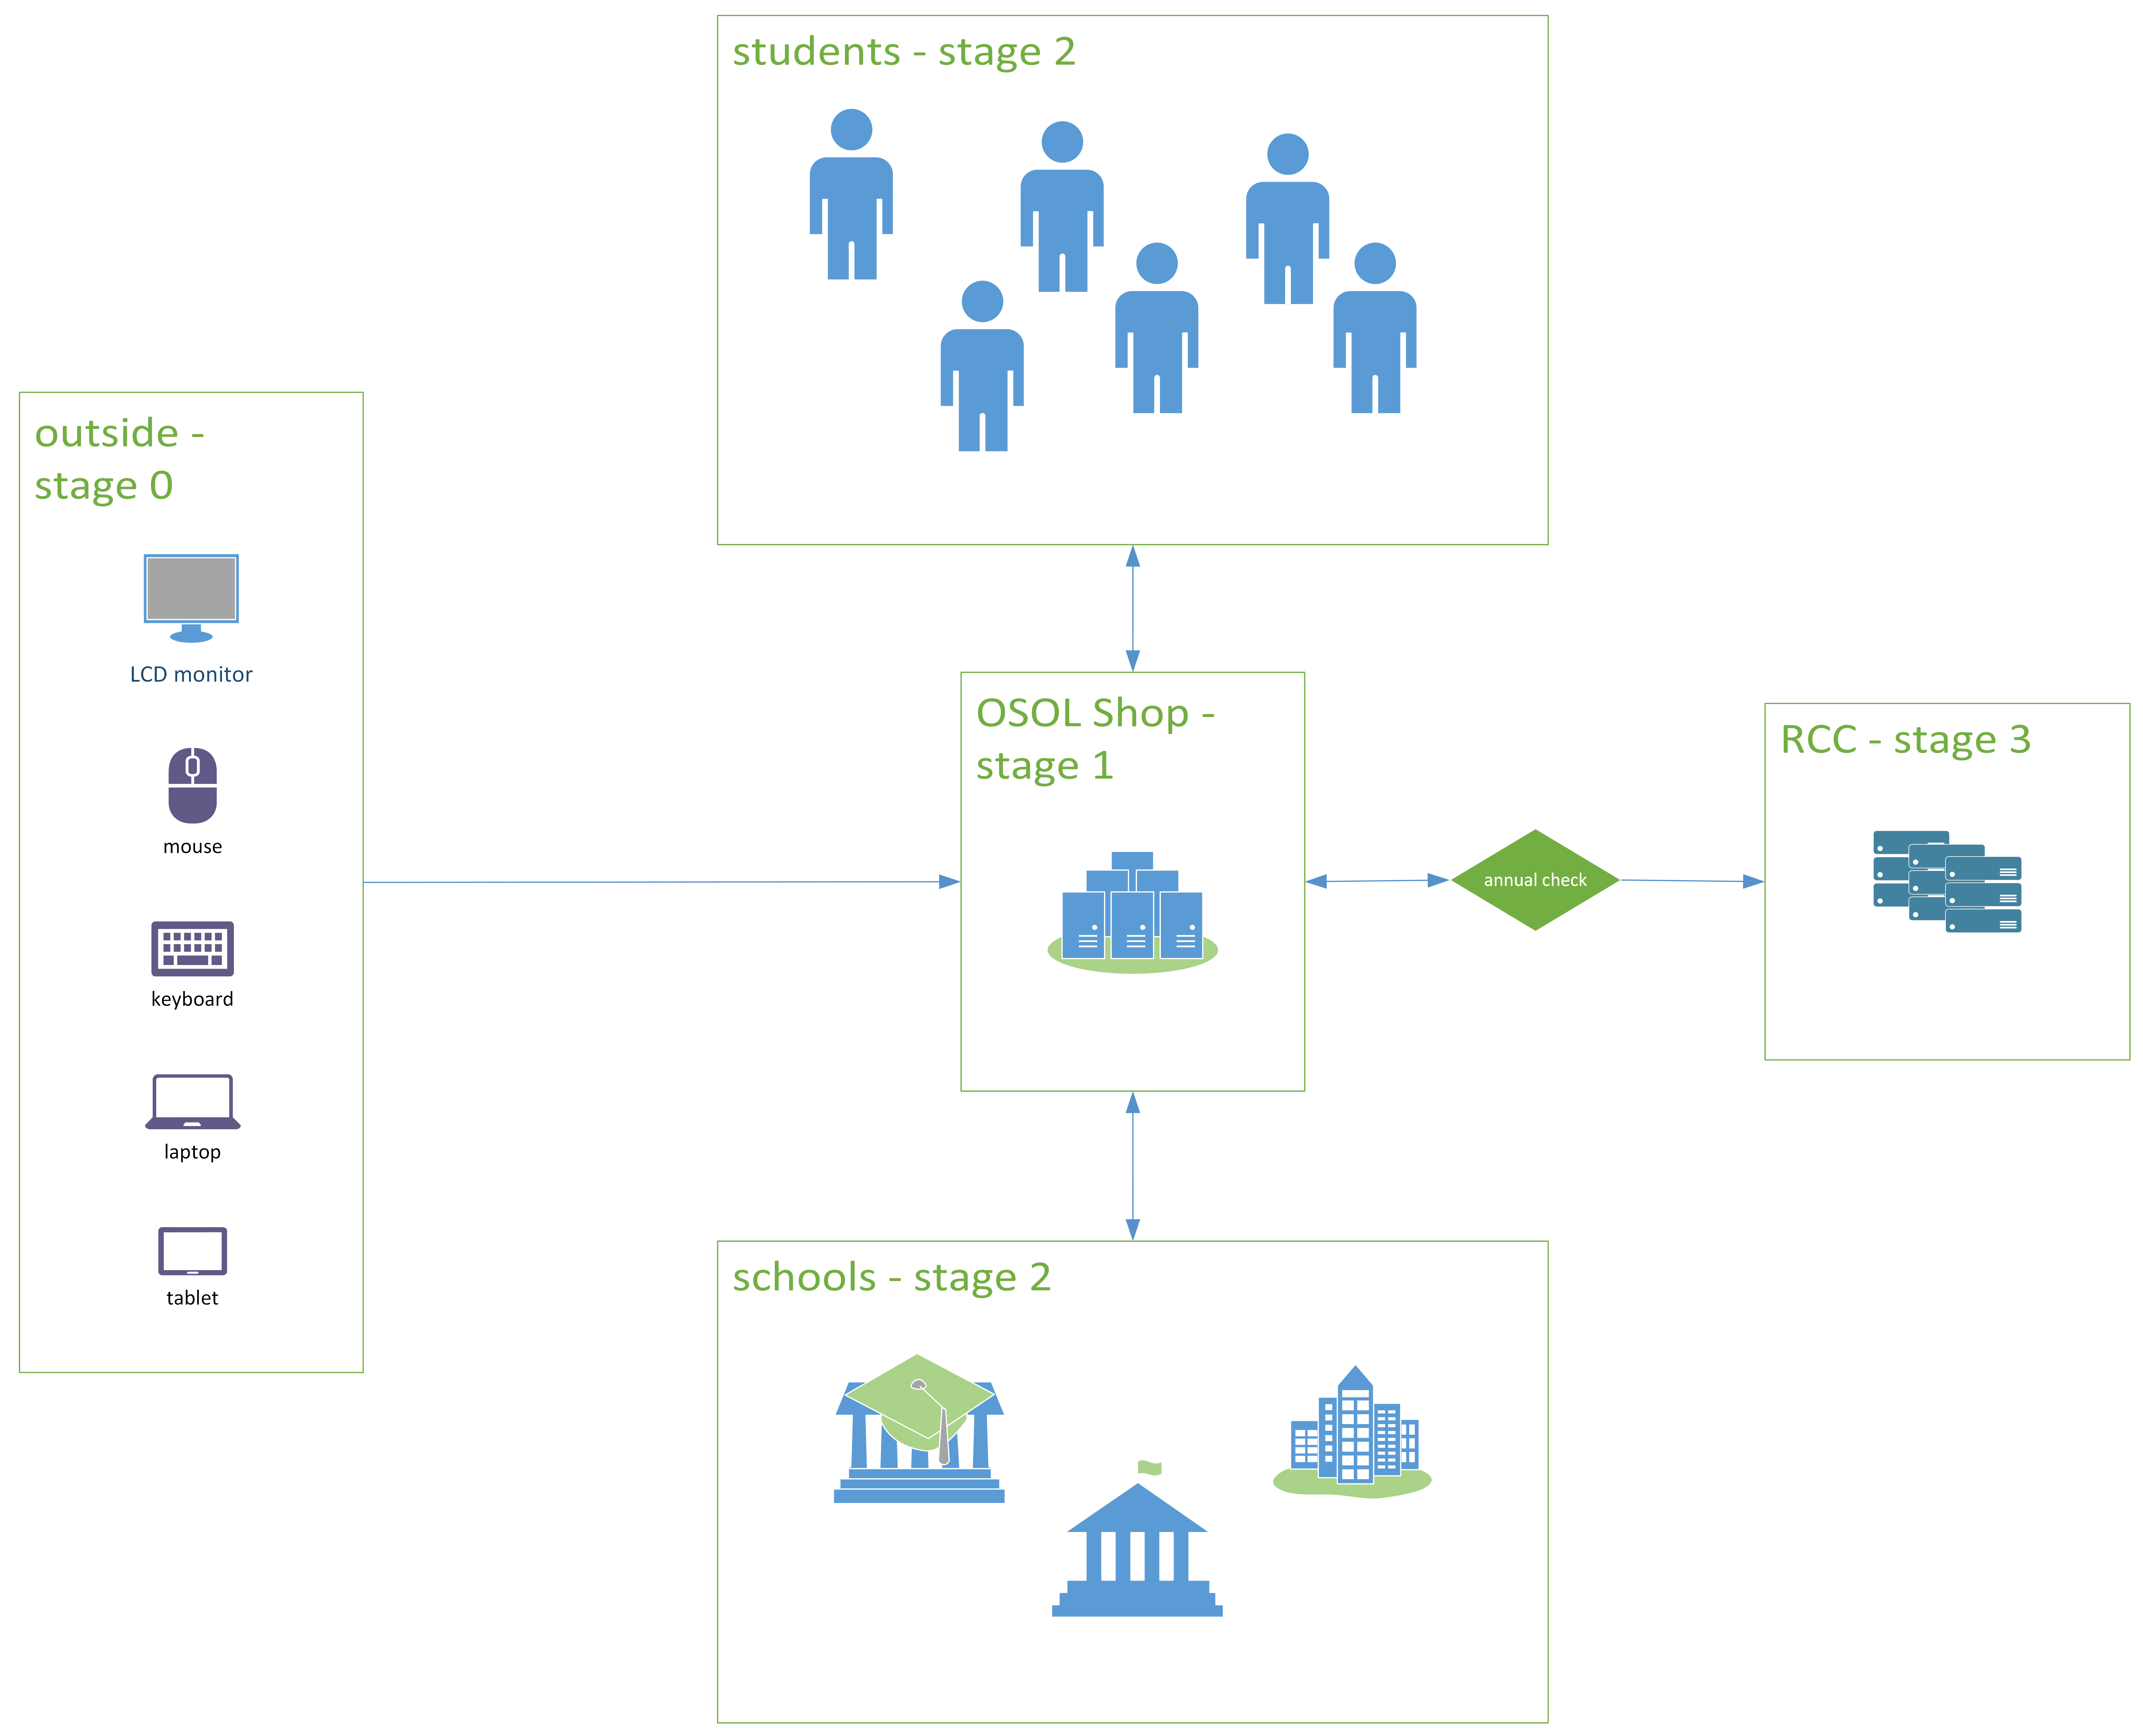
\includegraphics[width=0.9\linewidth]{osol-rcc}
	\caption{IT equipments lifecycle}
	\label{fig:osol-rcc}
\end{figure}


\subsubsection{Equipment stages}
\begin{enumerate}
	\item Stage 0 - outside OSOL

			
			
	\item Stage 1 - stay in OSOL Shop
		Hardware: disinfect, clean, basic repair
		Software: clean, install OS and needed education material, inspect
		
		
	\item Stage 2 - stay in student: less Grade6(12 years old) use Tablet, from Grade7(13 years old) start use Laptop.
	
	
	\item Stage 3 - stay in Reiverty Computer Center (RCC)
	

\end{enumerate}	

\subsubsection{Equipment score}

\subsubsection{Equipment annual check}

\subsection{OSOL 2D barcode  on IT equipment}

\subsubsection {Stage0 2D barcode data}
stick information list:
\begin{enumerate}
	\item strick\_print\_id
	\item equipment\_id
	\item from\_person\_id
	\item to\_person\_id
	\item action\_id
	\item action\_date
\end{enumerate}

\subsubsection {Stage1 2D barcode data}
stick information list:
\begin{enumerate}
	\item strick\_print\_id
	\item equipment\_id
	\item from\_person\_id
	\item to\_person\_id
	\item action\_id
	\item action\_date
	\item equipment\_score
	\item equipment\_info
\end{enumerate}

If equipment is Moniter, then equipment\_info list:
\begin{enumerate}
	\item brand
	\item model
	\item release\_date
	\item monitor\_type
	\item monitor\_resolution
	\item vga
	\item dvi
	\item dp
	\item hdmi
	\item usb\_c
	\item production\_date
\end{enumerate}

if equipment is Keyboard, then equipment\_info list:
\begin{enumerate}
	\item brand
	\item model
	\item release\_date
	\item is\_wireless
	\item is\_bluetooth
	\item is\_usb\_receiver
	\item key\_number
	\item keyboard\_type
	\item production\_date
\end{enumerate}

if equipment is Mouse, then equipment\_info list:
\begin{enumerate}
	\item brand
	\item model
	\item release\_date
	\item is\_wireless
	\item is\_bluetooth
	\item is\_usb\_receiver
	\item production\_date
\end{enumerate}

if equipment is Laptop or Tablet, then equipment\_info  list:
\begin{enumerate}
	\item brand
	\item model
	\item release\_date
	\item cpu\_info
	\item memory­\_type
	\item memory\_size(GB)
	\item gpu­\_info
	\item disk\_type
	\item disk\_size(GB)
	\item monitor­\_type
	\item monitor\_size(inch)
	\item monitor\_resolution
	\item is\_wifi
	\item is\_bluetooth
	\item usb\_a\_num
	\item usb\_c\_num
	\item hdmi\_num
	\item dp\_num
	\item vga\_num
	\item production\_date
\end{enumerate}

the cpu\_info list:
\begin{enumerate}
	\item cpu\_name
	\item manufacturer
	\item cores
	\item clock(GHz)
	\item L3\_cache(MB)
	\item release\_date
\end{enumerate}

the gpu\_info list:
\begin{enumerate}
	\item gpu\_name
	\item manufacturer
	\item gpu\_chip
	\item clock(GHz)
	\item gpu\_memory(MB)
	\item fp32(TFLOPS)
	\item release\_date
\end{enumerate}

\subsubsection {Stage2 2D barcode data}
stick information list:
\begin{enumerate}
	\item strick\_print\_id
	\item equipment\_id
	\item from\_person\_id
	\item to\_person\_id
	\item action\_id
	\item action\_date
\end{enumerate}

\subsubsection {Stage3 2D barcode data}
stick information list:
\begin{enumerate}
	\item strick\_print\_id
	\item equipment\_id
	\item from\_person\_id
	\item to\_person\_id
	\item action\_id
	\item action\_date
\end{enumerate}


\subsection{OSOL preinstalled education content}
\subsubsection{Math-desmos}
\href{https://www.desmos.com/}{Math-desmos}
\subsubsection{OpenAI ChatGPT}
\href{https://chatgpt.com/}{OpenAI ChatGPT}
\subsubsection{Google Gemini}
\href{https://gemini.google.com/}{Google Gemini}
\subsubsection{ResearchGate}
\href{https://www.researchgate.net/}{ResearchGatei}

	
\subsection{OSOL Tracer - OSOL Data Management System}
\subsubsection{OSOL-T Architecture}
\begin{figure}[h!]
	\centering
	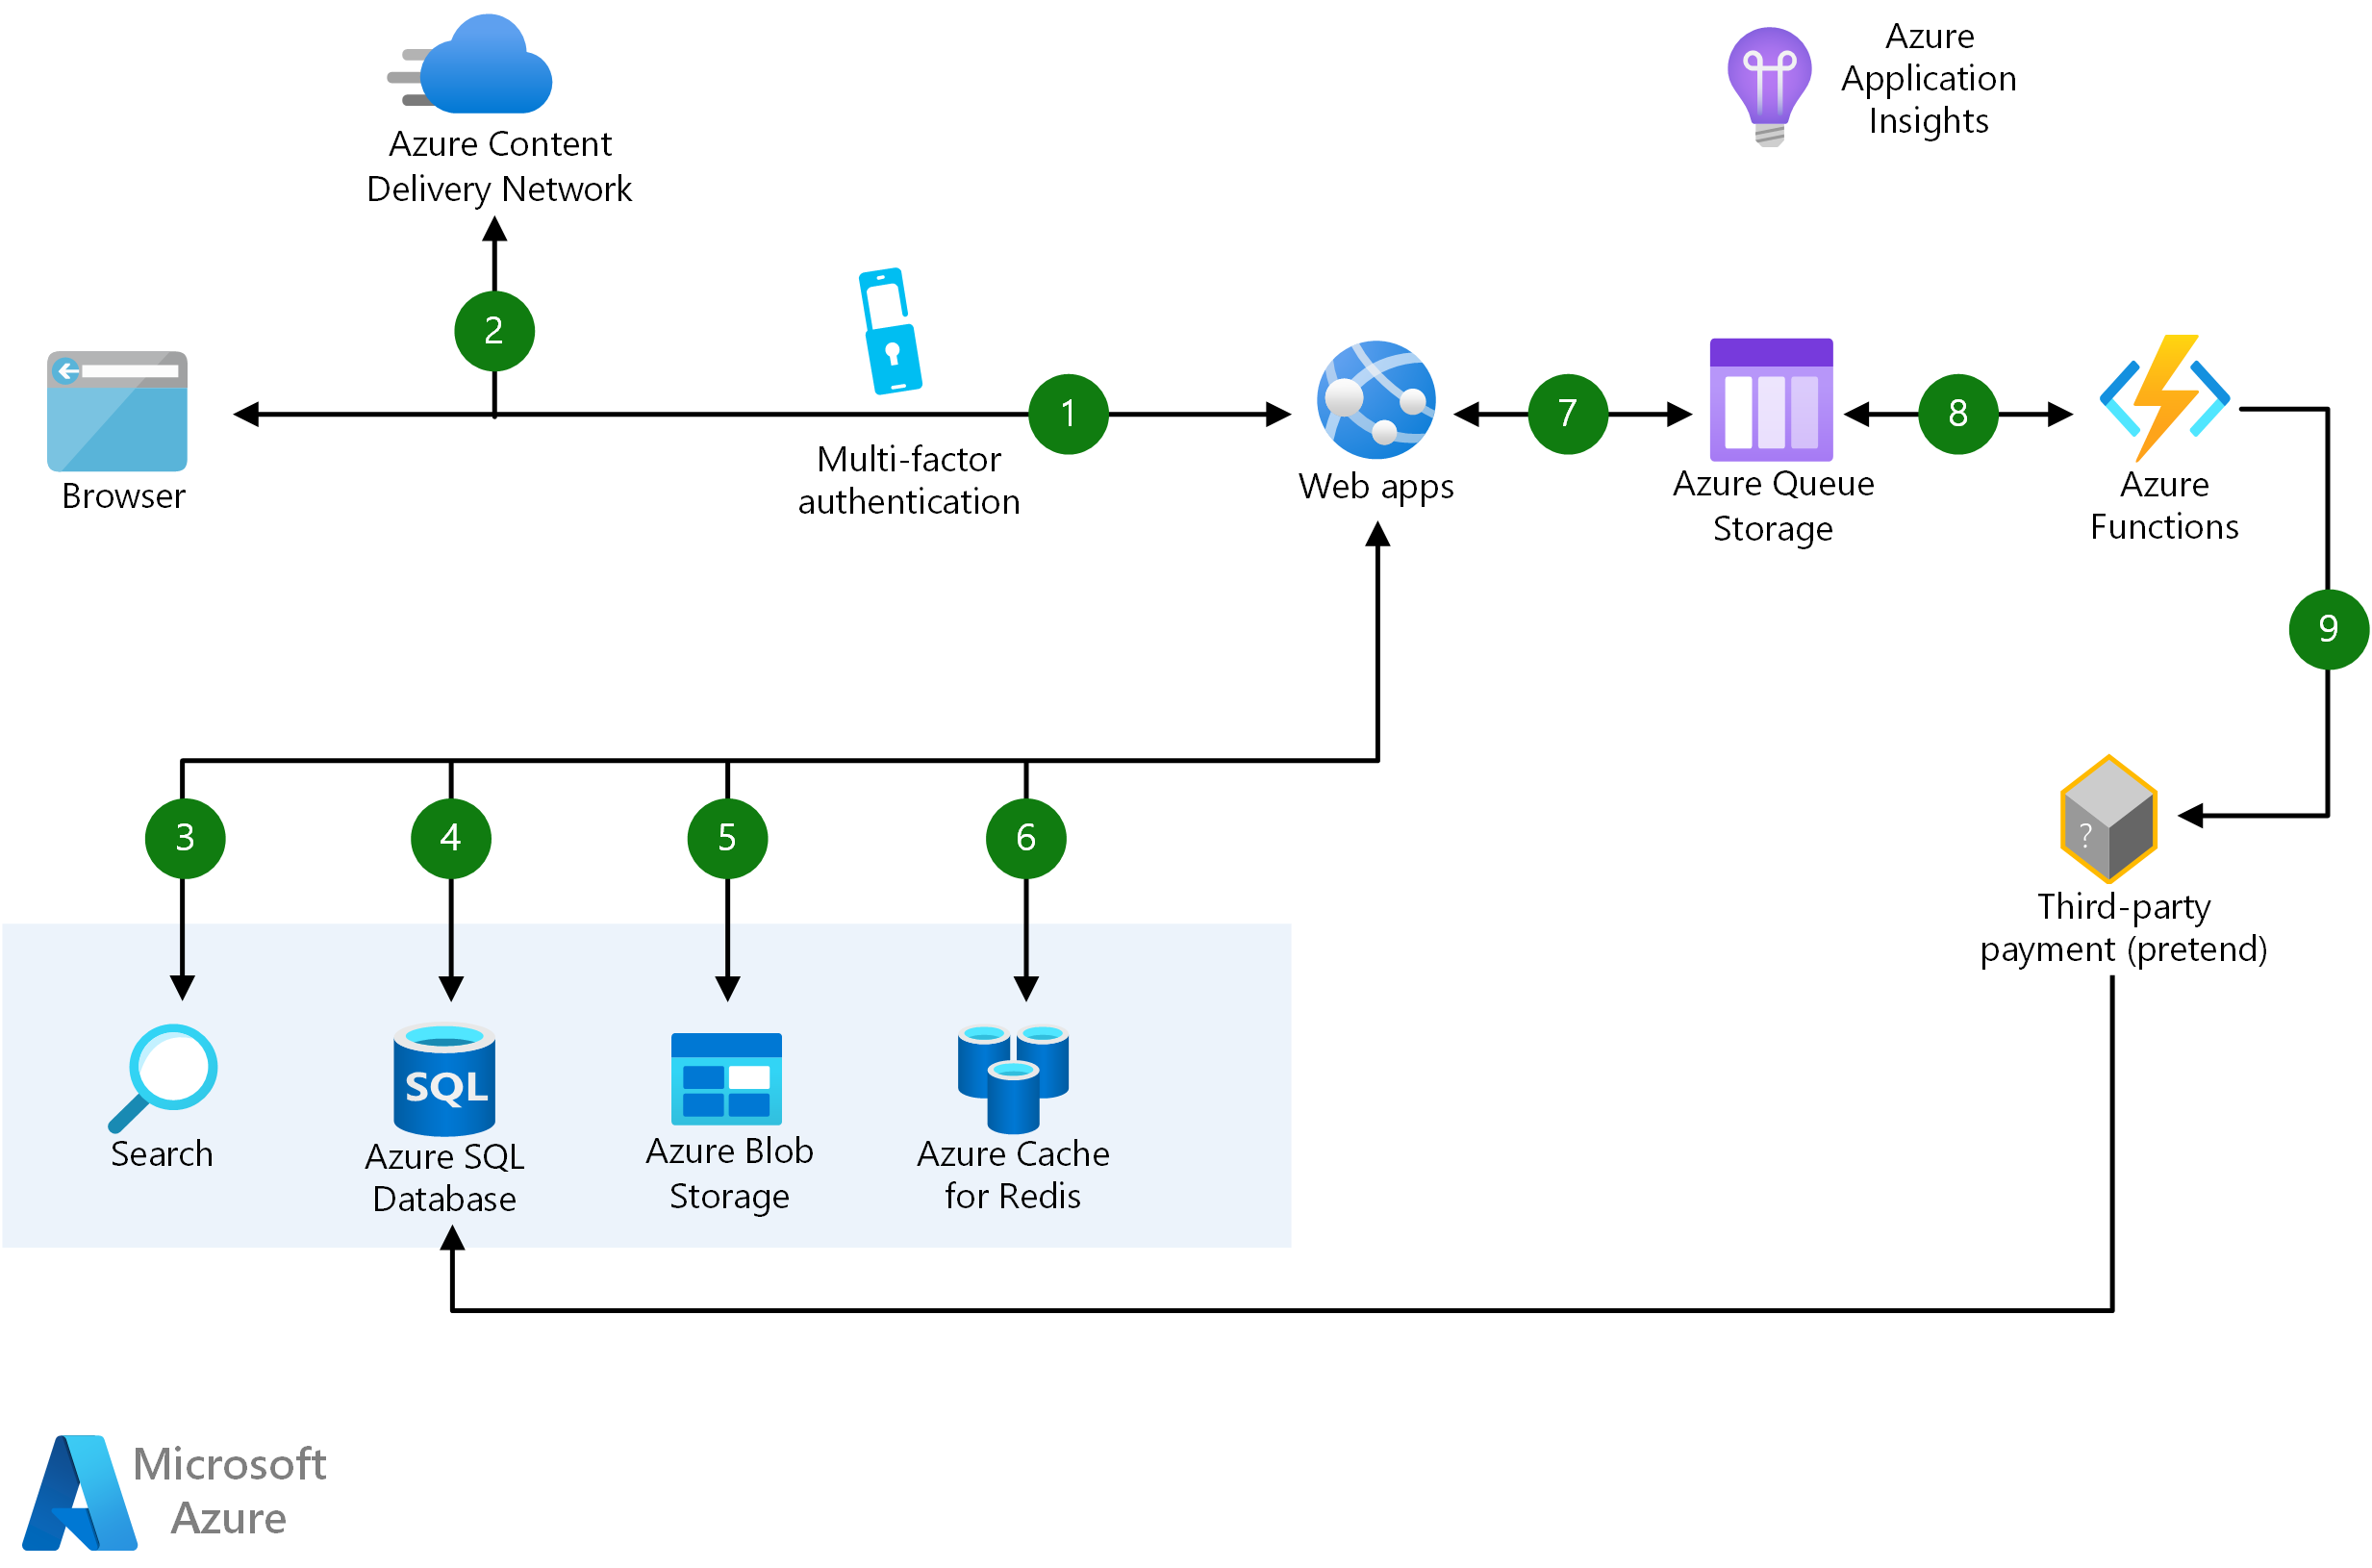
\includegraphics[width=0.9\linewidth]{scalable-ecommerce-web-app}
	\caption{OLPC Tracer Draft Architecture}
	\label{fig:scalable-ecommerce-web-app}
\end{figure}

{Why OSOL-T is serverless?}

\subsubsection{OSOL-T Database}
- relation database 
- MS Azure SQL Server
OSOL-T Database included below tables:
\begin{enumerate}
	\item osol.person
	\begin{enumerate}
		\item osol.address
		\item osol.communications
	\end{enumerate}
	\item osol.equipment
	\begin{enumerate}
		\item osol.laptop
		\item osol.monitor
		\item osol.mouse
		\item osol.keyboard
	\end{enumerate}
	\item osol.action
	\begin{enumerate}
		\item osol.action\_type
		\item osol.document
	\end{enumerate}
	\item stick\_print
\end{enumerate}
\subsubsection{OSOL-T API}
- Restful API for each databse object CRUD operations
- MS Azure Function 
\subsubsection{OSOL-T API Management }
\begin{figure}[h!]
	\centering
	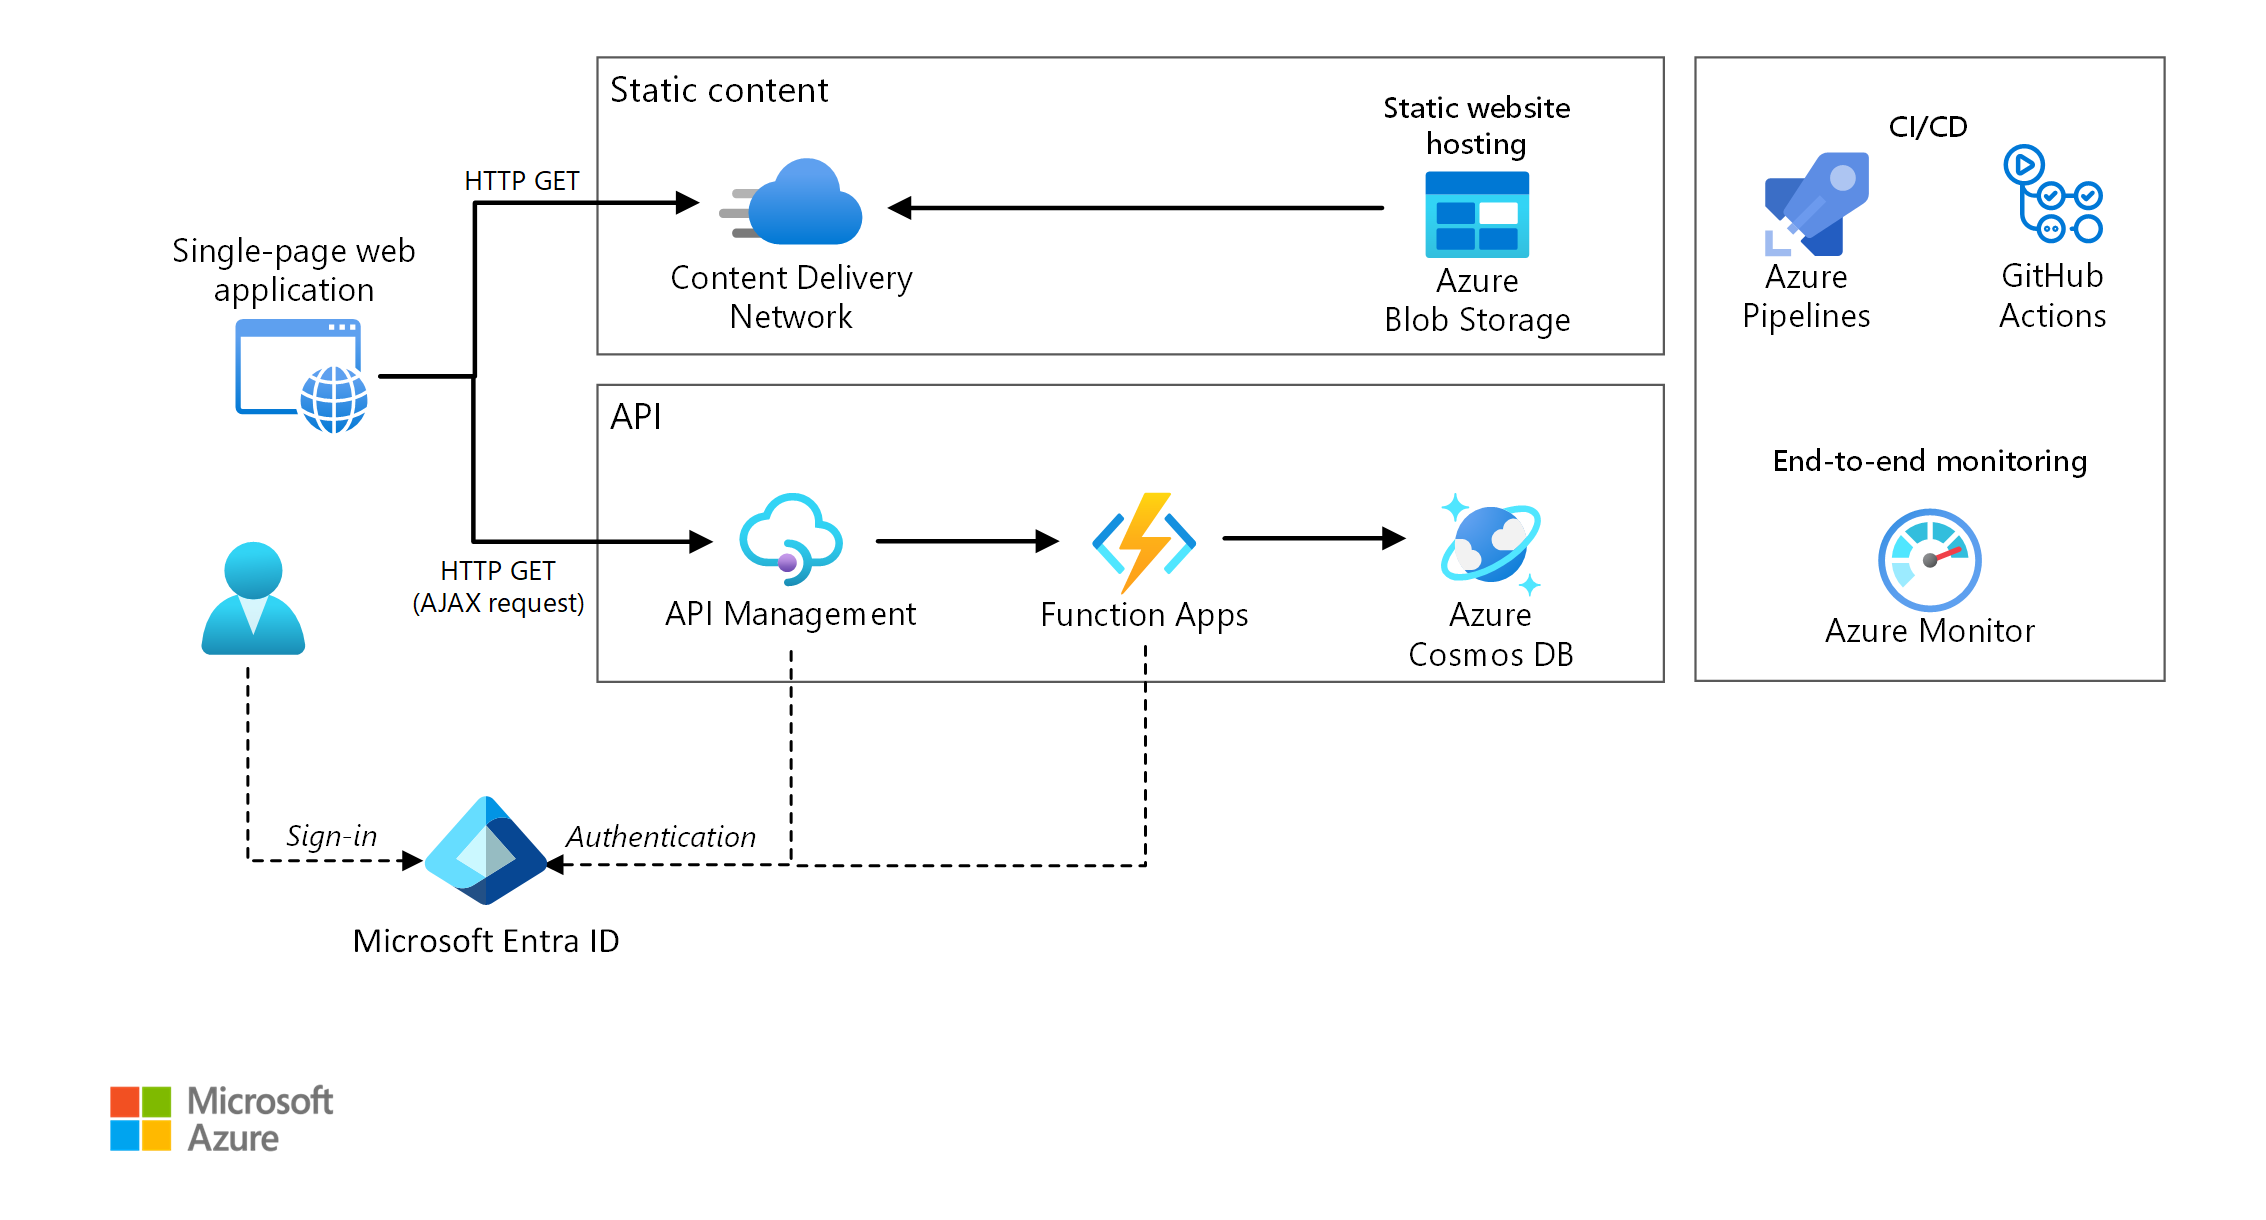
\includegraphics[width=0.9\linewidth]{serverless-web-app}
	\caption{MS Azure Serverless Architecture}
	\label{fig:serverless-web-app}
\end{figure}
\subsubsection{OSOL-T GUI}
OSOL-T GUI feature list:
\begin{enumerate}
	\item Multi-Platform - Mobile, Web - Flutter/Dart
	\item Input
	\item Search
	\item Print equipment stage 2D barcode
	\item Scan 2D barcode
	\item ChatBot
\end{enumerate}



\subsection{Riverty Computer Center(RCC)}
\begin{enumerate}
	\item RCC-abstract IO
	\item RCC-robust
	\item RCC-decentralization
	\item RCC-duplication and backup - data/process holographic : even $1/3$ computers are fail. $99.999\%$ data and computing process should be OK.
	\item RCC-hot plugging in Computer level
	\item RCC-AI based - ChatBot
\end{enumerate}


\section{When OSOL - Schedule}
\subsection{Step 1}
\begin{enumerate}
\item Just one place to store these out-of-date IT equipments.
\item Another guy to monitor and confirm each other with me.
\end{enumerate}

\section{OSOL Budget }

\appendix
\section{OSOL-T Database metadata}
\section{OSOL-T architecture - why use queue?}
\begin{enumerate}
	\item Decoupling
	\begin{itemize}
		\item Purpose: Queues act as a buffer between the API and the downstream services, such as databases or processing logic.
		\item Benefit: This ensures that the API can handle incoming requests without being directly tied to the speed or availability of the downstream services.
		\item Example: A user uploads data via an API, which places a message in a queue. The processing of the data happens asynchronously, allowing the API to quickly respond to the user.
	\end{itemize}
	\item Scalability
	\begin{itemize}
		\item Purpose: In serverless environments, the workload can spike unpredictably. A queue helps handle bursts of traffic by storing messages until they can be processed.
		\item Benefit: This allows your application to scale gracefully. For instance, Azure Functions or Logic Apps can process messages from the queue as they scale up or down automatically.
		\item Example: During high traffic, the queue can hold requests until Azure Functions has enough capacity to process them.
	\end{itemize}
	\item Reliability and Resilience
	\begin{itemize}
		\item Purpose: Queues ensure that no messages are lost, even if downstream services fail or experience downtime.
		\item Benefit: This helps in building fault-tolerant systems where messages are retried or processed later when the system recovers.
		\item Example: A queue can store order details submitted via an API. If the order-processing system crashes, the orders remain safe in the queue until the system is back online.
	\end{itemize}
	\item Throttling and Load Management
	\begin{itemize}
		\item Purpose: Queues help control the rate at which messages are processed by downstream services, preventing overload.
		\item Benefit: This protects the system from performance degradation or failures due to resource exhaustion.
		\item Example: The API can accept thousands of requests per second, but the backend may process only a hundred at a time. The queue enforces this limit.
	\end{itemize}
	\item Asynchronous Processing
	\begin{itemize}
		\item Purpose: Many tasks do not need to be performed immediately and can be handled in the background.
		\item Benefit: This improves the user experience by providing faster responses from the API and ensures better resource utilization.
		\item Example: An image-processing API can accept uploads quickly and push them to a queue. Processing, resizing, and storing the images happens asynchronously.
	\end{itemize}
	\item Retry and Dead-Letter Handling
	\begin{itemize}
		\item Purpose: Queues often support retries and dead-letter queues (DLQs) for failed messages.
		\item Benefit: If a message cannot be processed, it can be retried a set number of times, and if it still fails, it is moved to a DLQ for further investigation.
		\item Example: A payment processing API ensures no transaction request is lost. Failed requests are retried or stored in a DLQ.
	\end{itemize}
	\item Integration with Azure Services
	\begin{itemize}
		\item Azure provides built-in support for queues with services like Azure Queue Storage and Azure Service Bus. These services integrate seamlessly with Azure serverless components such as:
		\begin{itemize}
			\item Azure Functions: Triggered by queue messages to process tasks.
			\item Azure Logic Apps: Orchestrates workflows using queue messages.
			\item Azure Event Grid: Enables event-driven processing.
		\end{itemize}
	\end{itemize}
	
	\item Real-World Scenario
	For an e-commerce API:
	\begin{enumerate}
		\item A user places an order via the API.
		\item The order details are added to a queue.
		\item Downstream services like inventory checking, payment processing, and order confirmation process the queue messages asynchronously.
		\item If any service fails, the queue retains the message for retry or troubleshooting.
	\end{enumerate}
\end{enumerate}


%\begin{thebibliography}{99}

	%\bibitem{education-change-life-world}
	%\emph{How Education Can Change Your Life and the World: A Guide to Unlocking Your Potential and Fulfilling Your Purpose}. In {Araceli Aid Foundation}.  %\url{https://araceliaidfoundation.org/education/how-education-can-change-your-life-and-the-world-a-guide-to-unlocking-your-potential-and-fulfilling-your-purpose/}

	% Please avoid comments such as "For a review'', "For some examples",
	% "and references therein" or move them in the text. In general,
	% please leave only references in the bibliography and move all
	% accessory text in footnotes.
	
	% Also, please have only one work for each \bibitem.

%\end{thebibliography}

\bibliography{reference}{}
\bibliographystyle{plainurl}

\end{document}

